\documentclass[UTF8,11pt]{beamer}
\usepackage[utf8]{inputenc}
\usepackage{latexsym}
\usepackage[T1]{fontenc}
\usepackage{lmodern}
\usepackage[english]{babel}
\usepackage{amsmath}
\usepackage{amsfonts}
\usepackage{amssymb}
\usepackage{graphicx}
\usepackage{tikz}
\usetikzlibrary{matrix,shapes,arrows,positioning,fit,backgrounds,calc}
\usepackage{overpic}
\usepackage[]{algorithm}
\usepackage[]{algpseudocode} % noend
\usepackage[most]{tcolorbox}
\usepackage{ulem}
\usepackage{fancybox}
\usetikzlibrary{decorations.pathreplacing}
\usetheme{Eastlansing}
\newcommand{\fallingfactorial}[1]{%
	^{\underline{#1}}%
}
\mode<presentation>
\begin{document}
	\author{MA Jun}
	\title{Problem Solving}
	\subtitle{2-11 Heap \& Heapsort}
	\logo{
\includegraphics[width=0.05\textwidth]{figs/ICS_LOGO_left.png}}
	\institute{Institute of Computer Software}
	%\date{March 31, 2020}
	%\subject{}
	%\setbeamercovered{transparent}
	%\setbeamertemplate{navigation symbols}{}
\begin{frame}[plain]
	\maketitle
\end{frame}

\begin{frame}           %生成目录页,目录太长时加选项[shrink]
	\addtocounter{framenumber}{-2}%---------位置放在beginframe之后,不然无效
	\frametitle{Contents}
	\thispagestyle{empty}
	\tableofcontents[hideallsubsections]
\end{frame}
\AtBeginSection[]{
	\begin{frame}           %生成目录页,目录太长时加选项[shrink]
		\addtocounter{framenumber}{-1}%---------位置放在beginframe之后,不然无效
		\frametitle{Contents}
		\thispagestyle{empty}
		\tableofcontents[currentsection,hideallsubsections]
	\end{frame}
}
\section{Heaps}
\subsection{Basic Idea}

\begin{frame}
\centering{
	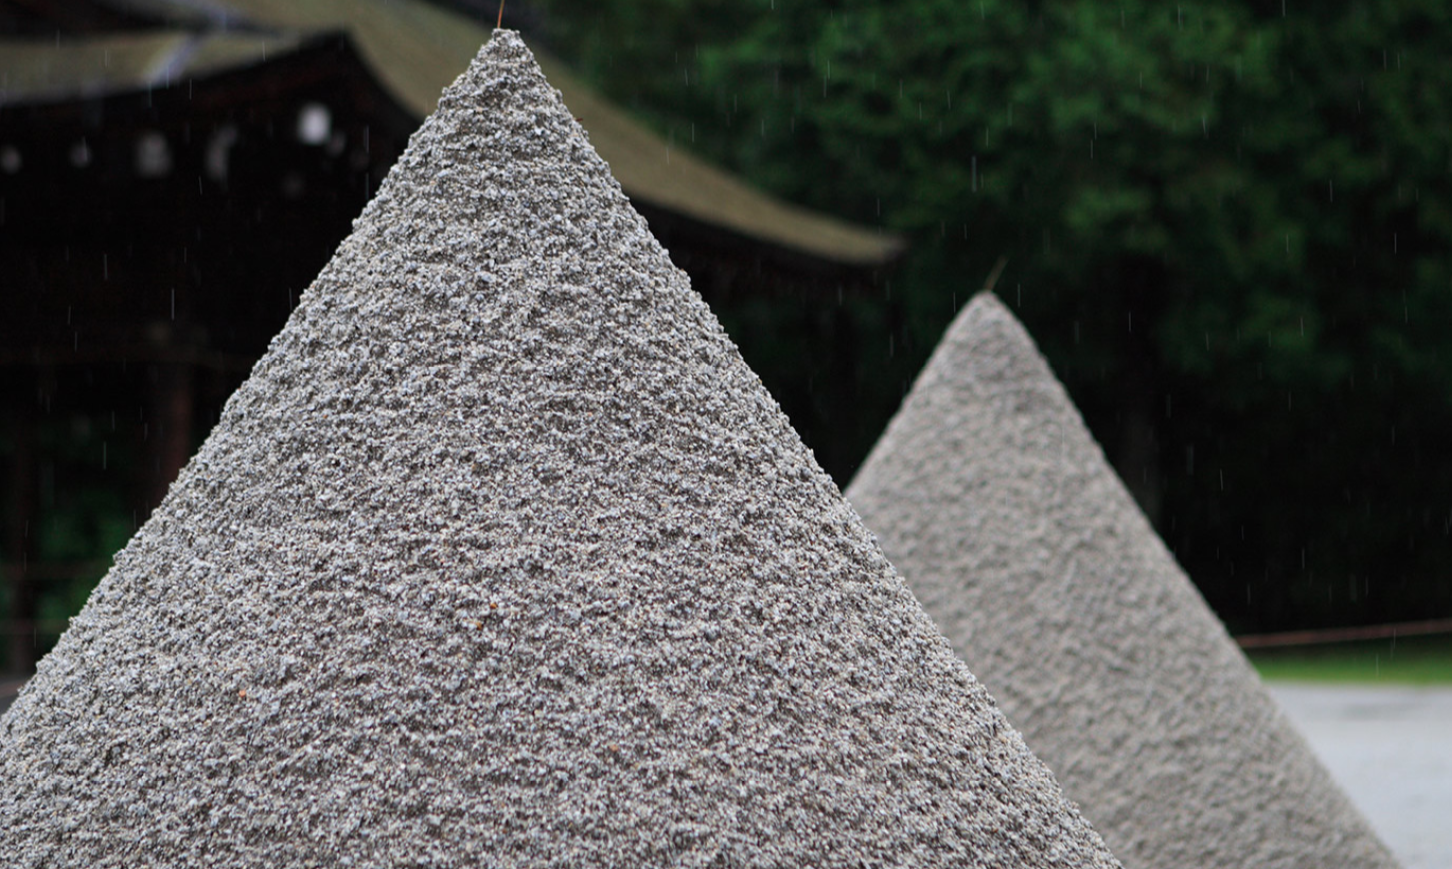
\includegraphics[width=0.4\linewidth]{figs/real_heap.png}
	
	Heap
}
\end{frame}

\begin{frame}           %生成目录页,目录太长时加选项[shrink]
\frametitle{Heaps}
\begin{block}{}
	The (binary) heap data structure is \textbf{\teal{an array object}} that we can view as a \textbf{\color{blue}nearly complete binary tree}
	\pause
	\begin{itemize}
		\item The tree is \teal{completely} filled on all levels {\color{blue}except possibly} the {\color{blue}lowest}
	\end{itemize} 
\end{block}
\begin{block}{}
	\begin{center}
	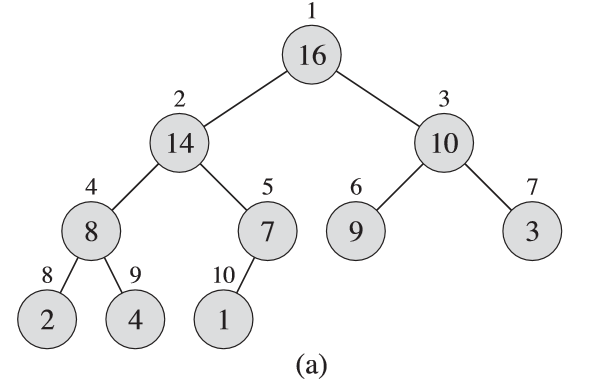
\includegraphics[width=.4\textwidth]{figs/heap_tree.png}
%	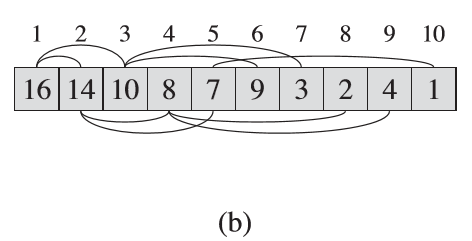
\includegraphics[width=.3\textwidth]{figs/heap_array.png}
%	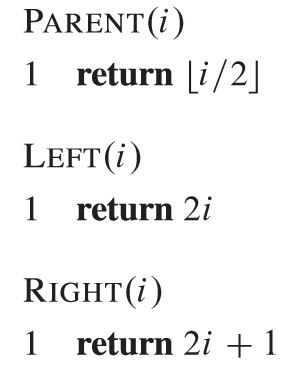
\includegraphics[width=.2\textwidth]{figs/heap_array_parent_procedure.png}
	\end{center}
	
\end{block}
\end{frame}

\begin{frame}           %生成目录页,目录太长时加选项[shrink]
\frametitle{Heaps: Max-heap VS Min-heap}
\begin{columns}
	\begin{column}[T, onlytextwidth]{.45\textwidth}
	\begin{center}
		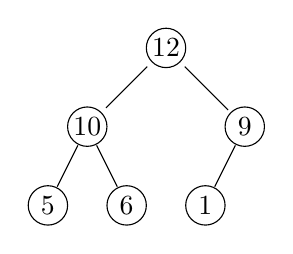
\begin{tikzpicture}
		\draw [] (0,0) node (a){12} circle (0.25cm);
		\draw [] (-1,-1) node (b){10} circle (0.25cm);
		\draw [] (1,-1) node (c){9} circle (0.25cm);
		\draw [] (-1.5,-2) node (d){5} circle (0.25cm);
		\draw [] (-0.5,-2) node (e){6} circle (0.25cm);
		\draw [] (0.5,-2) node (f){1} circle (0.25cm);
		\draw (a)--(b);
		\draw (a)--(c);
		\draw (b)--(d);
		\draw (b)--(e);
		\draw (c)--(f);
		\end{tikzpicture}
		\begin{block}{Max-heap property}
			\begin{center}
			$A\left[ Parent(i)\right]\ge A\left[ i\right]  $
			\end{center}	
		\end{block}
	\end{center}
	\end{column}
	\begin{column}[T, onlytextwidth]{.45\textwidth}
		\begin{center}
		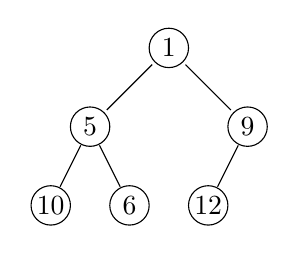
\begin{tikzpicture}
		\draw [] (0,0) node (a){1} circle (0.25cm);
		\draw [] (-1,-1) node (b){5} circle (0.25cm);
		\draw [] (1,-1) node (c){9} circle (0.25cm);
		\draw [] (-1.5,-2) node (d){10} circle (0.25cm);
		\draw [] (-0.5,-2) node (e){6} circle (0.25cm);
		\draw [] (0.5,-2) node (f){12} circle (0.25cm);
		\draw (a)--(b);
		\draw (a)--(c);
		\draw (b)--(d);
		\draw (b)--(e);
		\draw (c)--(f);
		\end{tikzpicture}
		\begin{block}{Min-heap property}
			\begin{center}
			$A\left[ Parent(i)\right]\le A\left[ i\right]  $
			\end{center}
		\end{block}
		\end{center}
	\end{column}
\end{columns}
\end{frame}

\begin{frame}           %生成目录页,目录太长时加选项[shrink]
\frametitle{Heaps: Storage}
\question{1}{Why do we implement a heap with an array?}

\begin{block}{}
	\begin{center}
		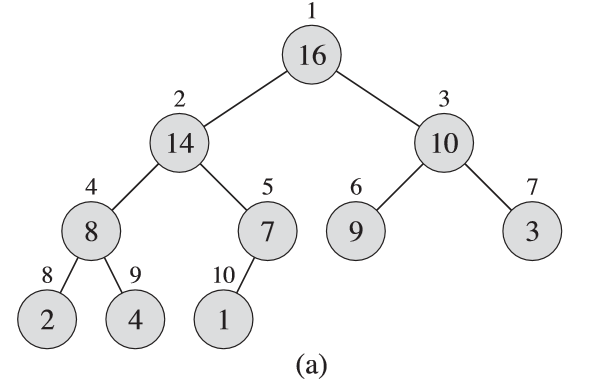
\includegraphics[width=.4\textwidth]{figs/heap_tree.png}
		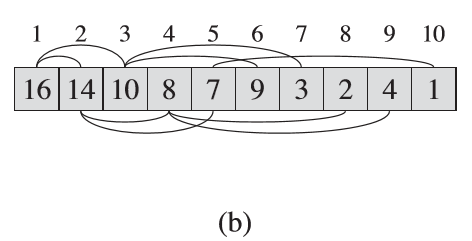
\includegraphics[width=.3\textwidth]{figs/heap_array.png}
		\onslide<2->{
			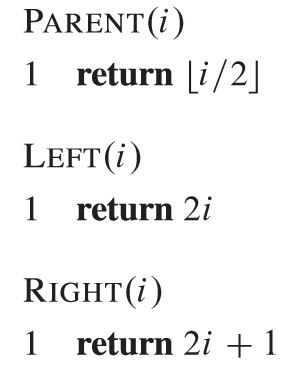
\includegraphics[width=.2\textwidth]{figs/heap_array_parent_procedure.png}
		}
	\end{center}
\begin{itemize}
	\onslide<2->{
		\item Easy to index
	}
	\onslide<3->{
		\item Save memory
	}
	\onslide<4->{
		\item Better cache locality
	}
\end{itemize}
\end{block}
\end{frame}

\begin{frame}           %生成目录页,目录太长时加选项[shrink]
\frametitle{Heaps: Height}
\begin{block}{The height of a node}
	\begin{itemize}
		\item The number of edges on the \teal{longest simple downward path} from the node to a leaf.
	\end{itemize}
	 
\end{block}

\pause
\begin{block}{The height of a heap}
	\begin{itemize}
		\item The height of its root, {\color{blue}$\Theta(\lg{n})$}.
		\item A heap of $n$ elements is based on a \textbf{nearly complete binary tree}
	
	\end{itemize}
\end{block}
\begin{block}{}
	\begin{center}
		\begin{tikzpicture}
			\node at (0,0){
				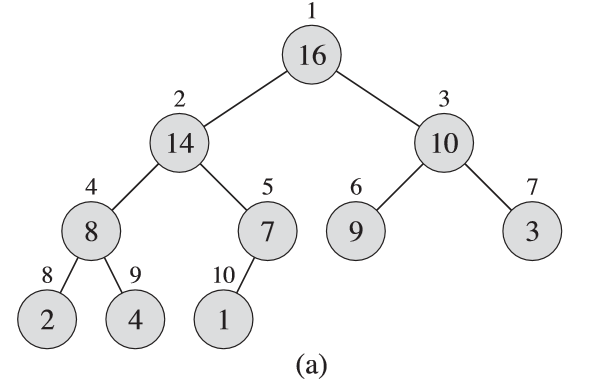
\includegraphics[width=.4\textwidth]{figs/heap_tree.png}};
			\footnotesize{
				\node at(0.7,1.2){h=3};
				\node at(1.7,0.5){h=1};
				
				\node at(-1.7,0.5){h=2};
				
				\node at(2.3,-0.2){h=0};
				\node at(-2.3,-0.2){h=1};
				
				\node at(0,-0.9){h=0};
			}
		\end{tikzpicture}
	\end{center}
\end{block}
\end{frame}


\begin{frame}
\frametitle{Heaps: basic operations}
\begin{block}{}
	\begin{tikzpicture}
		\node at(0,0) {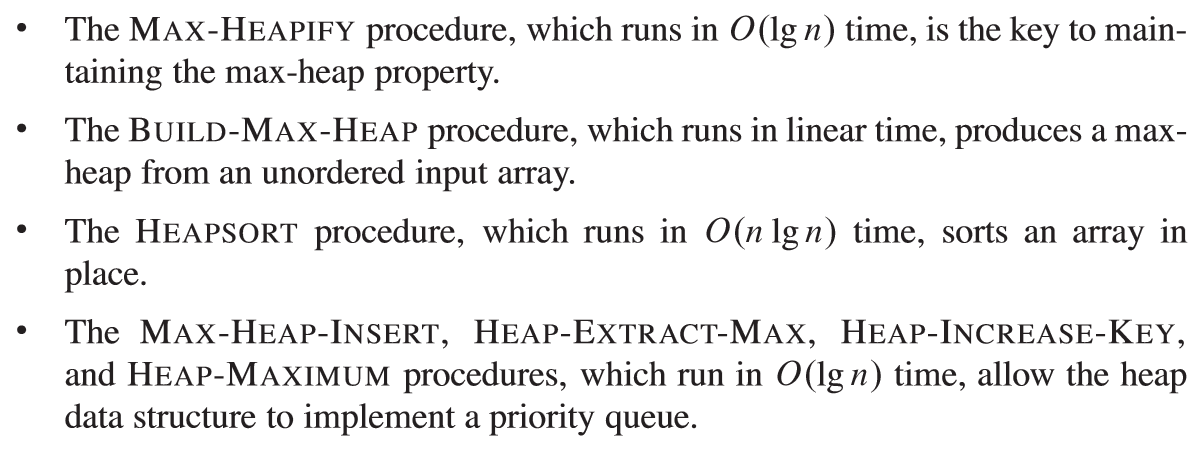
\includegraphics[width=0.9\textwidth]{figs/operations_on_heap.PNG}};
			\coordinate (c1l) at(-4.3,1.8);
		\coordinate (c1r) at(-2.2,1.8);
		\coordinate (c2l) at(-4.3,0.9); 
		
		\coordinate (c3l) at(-4.3,-0.9); 
		\coordinate (c3t) at(-2.85,-0.7);
		
		\coordinate (c4t) at(0.5,-0.7);
		
		\coordinate (c5t) at(3.75,-0.7);
		
		\pause
		\draw [color=blue,thick] (-4.3,1.6) rectangle +(2.1,0.4);
		\pause
		\draw [color=blue,thick] (-4.3,0.7) rectangle +(2.7,0.4);
		\draw [color=blue,->, >=triangle 45] (c2l).. controls (-5,0.9) and (-5,1.8)..(c1l);
		\pause
		\draw [color=red,thick] (-4.3,-0.2) rectangle +(1.6,0.4);
		
		\pause
		\draw [color=blue,thick] (-4.3,-1.1) rectangle +(2.9,0.4);
		\draw [color=blue,thick] (-1.2,-1.1) rectangle +(3.1,0.4);
		\draw [color=blue,thick] (2.1,-1.1) rectangle +(3.3,0.4);
		\draw [color=blue,thick] (-4.3,-1.55) rectangle +(2.5,0.4);
		
		\pause
		\draw [color=blue,->, >=triangle 45] (c3t).. controls (-2.85,0) and (3.75,0)..(c5t);
		\draw [color=blue,->, >=triangle 45] (c4t).. controls (-2,0.5) and (3,0.5)..(c1r);	
		\pause
		\draw [color=red,thick] (-1.1,-2) rectangle +(2,0.4);
	\end{tikzpicture}
	
\end{block}
\end{frame}
\subsection{Maintaining the heap property}
\begin{frame}
\frametitle{ Maintaining the heap property: \textproc{Max-Heapify}}
\begin{center}
	\question{2}{ Can you explain the process of \textproc{Max-Heapify}}
		\begin{center}
			\begin{tikzpicture}
				\node at(0,0){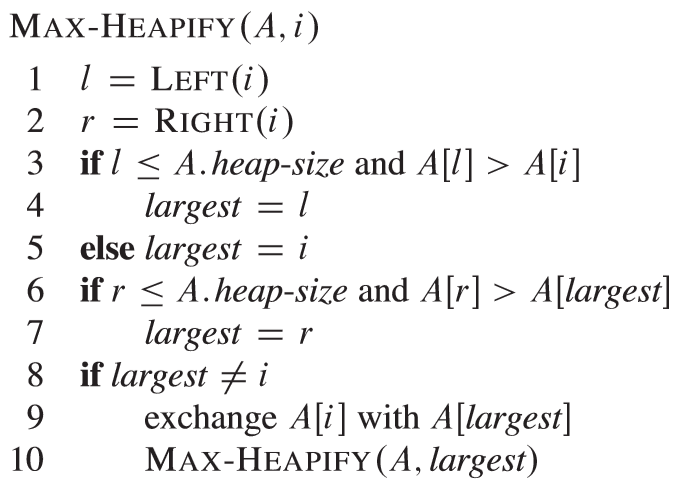
\includegraphics[width=0.45\textwidth]{figs/MAX-HEAPIFY.PNG}};
				
				
				
				\pause
				\draw [color=red,thick] (-2.2,0.8) rectangle (-0.3,1.5)node(a){};
				\node (b)at (4,1.5) [fill= green!50!black!20!,text width=7cm]{ \footnotesize{\textbf{\color{blue}Pre-condition:}$Left(i)$ and  $Right(i)$ are maxheaps.}};
				\node (e)at (6,0.5) [fill= green!50!black!20!,text width=5cm]{ \footnotesize{\textbf{\color{blue}Post-condition:}the tree rooted at $i$ is a maxheap.}};
				
				\draw [color=red,->,thick] (b)--(a);
				
				\pause
				\draw [color=red,thick] (-1.85,-1.2) rectangle +(0.9,0.3);
				\node (c) at (5,-1) [fill= green!50!black!20!,text width=4cm]{ \footnotesize{\parbox{4cm}{index of the largest element in the tree rooted at $i$}}};
				
				\draw [color=gray,thick] (-2.2,-1.2) rectangle +(5,2);
				
				\pause
				\draw [color=blue,thick] (-1.6,-1.9) rectangle (1.5,-1.45);
			\end{tikzpicture}
			
		\end{center}
	
	
	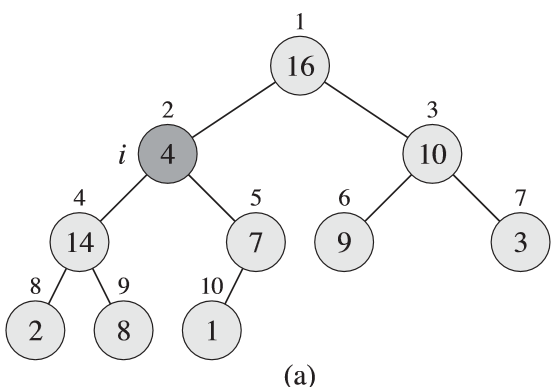
\includegraphics[width=0.32\textwidth]{figs/MAX-HEAPIFY(a).PNG}
	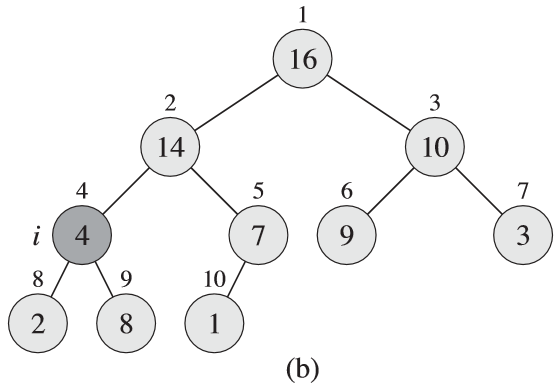
\includegraphics[width=0.32\textwidth]{figs/MAX-HEAPIFY(b).PNG}
	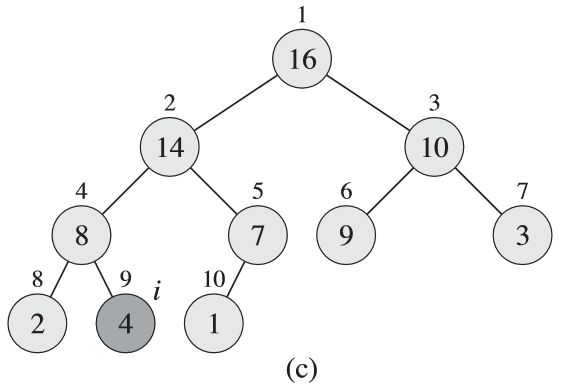
\includegraphics[width=0.32\textwidth]{figs/MAX-HEAPIFY(c).PNG}
\end{center}
\end{frame}

\begin{frame}
\frametitle{ Maintaining the heap property: \textproc{Max-Heapify}}
\begin{center}
	\begin{block}{\textbf{\color{blue}Worst-case} for \textproc{Max-Heapify}}
	\begin{columns}
	\begin{column}[T]{0.45\textwidth}
			
		\begin{center}
			\begin{tikzpicture}
			\node at(0,0){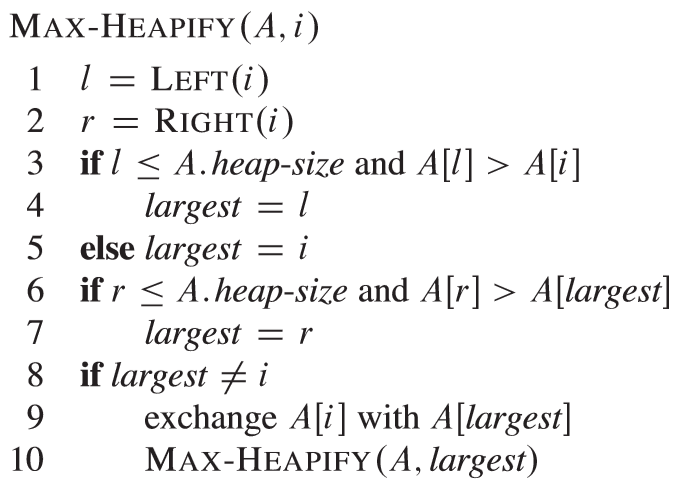
\includegraphics[width=\textwidth]{figs/MAX-HEAPIFY.PNG}};
			
			\onslide<2>
			\draw [color=gray,thick] (-2.2,-1.2) rectangle +(5,2);
			\onslide<3>
			\draw [color=blue,thick] (-1.6,-1.9) rectangle (1.5,-1.45);
			\end{tikzpicture}
			
		\end{center}

		\end{column}	
		\begin{column}[T]{0.5\textwidth}
			The running time of \textproc{Max-Heapify} on a subtree of size $n$ rooted at a given node $i$ is the sum of:
			\begin{itemize}
				
			\onslide<2->{	\item  Time to find the \teal{largest}, {\color{green}$\Theta(1)$}}
			
			\onslide<3->{	\item Time to run \textproc{Max-Heapify} recursively, $\le {\color{red}T(2n/3)}$}
			\end{itemize}
		
		\end{column}
	\end{columns}
	\end{block}	
	\onslide<4->{
		\fbox{\color{blue}$T(n)\le {\color{red}T(2n/3)}+{\color{green}\Theta(1)}=O(\lg{n})\onslide<4->{=O(h)}$}
	}
\end{center}
\end{frame}

\begin{frame}
\frametitle{ Maintaining the heap property: \textproc{Max-Heapify}}

\begin{block}{\textbf{\color{blue}Worst-case} for \textproc{Max-Heapify}}
	\begin{center}
		Time to run \textproc{Max-Heapify} recursively, $\le {\color{red}T(2n/3)}$
		\vspace{0.3cm}
		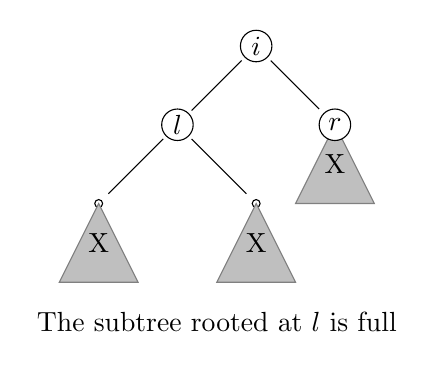
\begin{tikzpicture}
			\onslide<2->
			\filldraw [fill=white](0,0) circle  (0.2) node(n1){$i$};
			
			\filldraw [fill=white](-1,-1) circle  (0.2) node(n2){$l$};
			\filldraw [gray,fill=lightgray] (1,-1)--(0.5,-2)--(1.5,-2)--cycle;
			\filldraw [fill=white](1,-1) circle  (0.2) node(n3){$r$};
			\filldraw [fill=white](-2,-2) circle  (0.05) node(n4){ };
			\filldraw [fill=white](0,-2) circle  (0.05) node(n5){ };
			\draw (n1)--(n2);
			\draw (n1)--(n3);
			
			\filldraw [gray,fill=lightgray] (-2,-2)--(-2.5,-3)--(-1.5,-3)--cycle;
			\filldraw [gray,fill=lightgray] (0,-2)--(-0.5,-3)--(0.5,-3)--cycle;
			\draw (n2)--(n4);
			\draw (n2)--(n5);
			
			\onslide<3->
			\node at (-0.5,-3.5) {The subtree rooted at $l$ is full};
			%number of nodes in subtrees
			\onslide<4->
			\node at(-2,-2.5) {X};
			\node at(0,-2.5) {X};
			\node at(1,-1.5) {X};
		\end{tikzpicture}
		\begin{itemize}
		\onslide<5->{	\item  Total number of nodes $n=3X+2$}
		\onslide<6->{	\item  Total number of nodes in the left subtree $2X+1$}
		\onslide<7->{	\item  $\frac{2X+1}{3X+2}<2/3$}
		\end{itemize}
	\end{center}
\end{block}	
\end{frame}

\subsection{Building a heap}
\begin{frame}
\frametitle{Building a heap: \textproc{Build-Max-Heap}}
\begin{center}
	\begin{columns}
		\begin{column}[T]{0.4\textwidth}
			\question{3}{ Can you explain the process of \textproc{Build-Max-Heap}}	
				\begin{center}
					\begin{tikzpicture}
					\node at (0,0) {	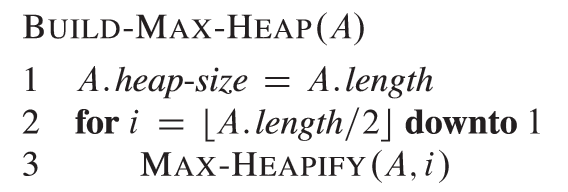
\includegraphics[width=\textwidth]{figs/BUILD-MAX-HEAP_procedure.png}				};
					\onslide<2->{
						\draw [color=red,thick](-1.4,-0.4) rectangle +(2.4,0.4);
					}
					\end{tikzpicture}
				
				\end{center}
			
			\onslide<4->{
				\question{4}{Can you prove the correctness of \textproc{Build-Max-Heap}?}
			}
		\end{column}
		\begin{column}[T]{0.55\textwidth}
			\begin{tikzpicture}
				\node at(0,0){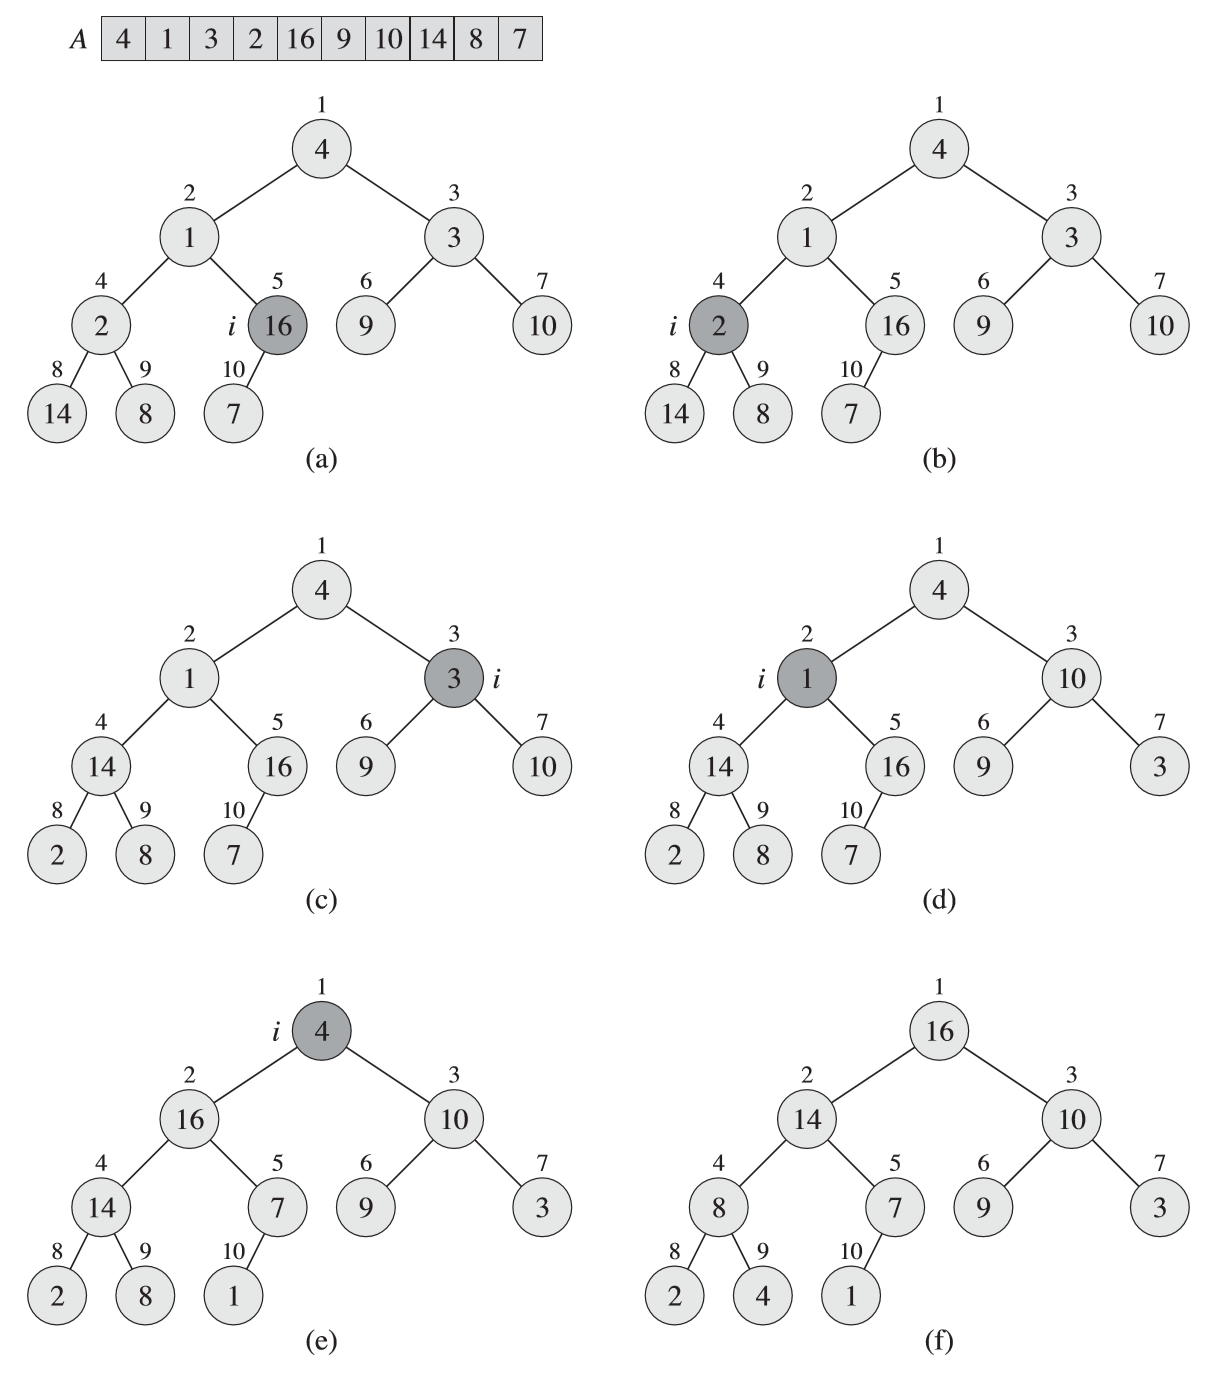
\includegraphics[width=0.9\textwidth]{figs/BUILD-MAX-HEAP_example.png}};
				\onslide<2->{
					\draw [color=red,thick] (-1.4,3.4)--(-1.4,3);
				}
				\onslide<3->{
					\draw [dashed,color=blue](-3,1.6)--(-1.4,1.6)--(-1.4,2)--(0,2)--(0,1.5)--(-1.2,1.5)--(-1.2,1.1)node[below]{\footnotesize{one-element heaps}}--(-3,1.1)--cycle ;
				}
			\end{tikzpicture}
				
		\end{column}
	\end{columns}
\end{center}
\end{frame}

\begin{frame}
\frametitle{Correctness of \textproc{Build-Max-Heap}}
\begin{center}
\begin{block}{Invariant}
\teal{	At the start of each iteration of the for loop of lines 2-3, each node $i+1,i+2,\cdots,n$ is the root of a max-heap. }
\end{block}

\pause
\begin{proof}
	\begin{tikzpicture}
		\node at(0,0) {	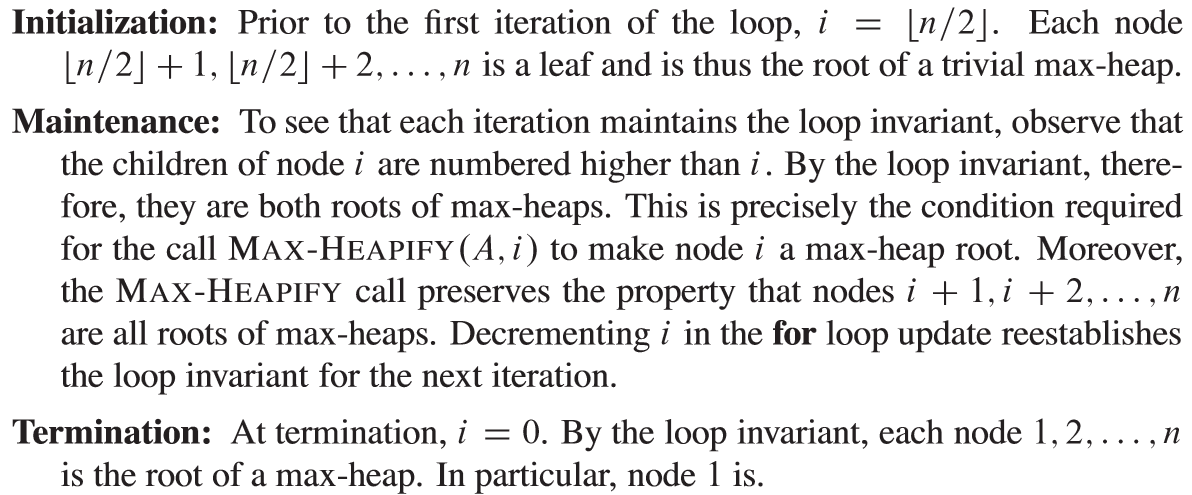
\includegraphics[width=0.9\textwidth]{figs/proof_correctness_build_max_heap.png}};
	\pause	
		\draw [color=red,thick] (-5,1.5)--(0,1.5);
	\pause	
		\draw [color=red,thick] (-3.4,-0.2)--(-0.5,-0.2);
	\pause
		\draw [color=red,thick] (-1.4,-1.8)--(-0.4,-1.8);
	\end{tikzpicture}
\end{proof}
\end{center}
\end{frame}
\begin{frame}[t]
\frametitle{Running time of \textproc{Build-Max-Heap}}
\begin{center}
	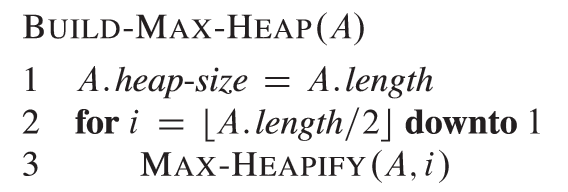
\includegraphics[width=0.5\textwidth]{figs/BUILD-MAX-HEAP_procedure.png}
	
	\pause
	\begin{block}{A poor upper bound}
		\begin{itemize}
			\item Each call to \textproc{ Max-Heapify} costs $O(\lg{n})$
			\item At most $O(n)$ calls
			\item Thus, \textbf{\color{blue}$O(n\lg{n})$}
		\end{itemize}
	\end{block}
	
	\pause
	\question{5}{Can you give a better one?}
\end{center}
\end{frame}

\begin{frame}[t]
\frametitle{Running time of \textproc{Build-Max-Heap}}
\begin{center}
	\begin{block}{A tighter linear upper bound}
		\begin{itemize}
			\pause
			\item An $n$-element heap has height {\color{teal}$\lfloor\lg{n}\rfloor$}.
			
			\pause
			\item At most {\color{teal}$\lceil n/{2^{h+1}}\rceil$} nodes of any height $h$.
			
			\pause
			\item Thus,
			\[
				\sum\limits_{h=0}^{\lfloor\lg{n}\rfloor}{\lceil\frac{n}{2^{h+1}}\rceil O(h)}
				\pause
				=O\left(n \sum\limits_{h=0}^{\lfloor\lg{n}\rfloor}{\frac{h}{2^h}}\right)\pause
				=O\left(n \sum\limits_{h=0}^{\infty}{\frac{h}{2^h}}\right)
				={\color{blue}O(2n)}
				={\color{blue}O(n)}
			\]
			
			\pause
			\centering{\teal{\fbox{
				$
				\sum\limits_{h=0}^{\lfloor\lg{n}\rfloor}{\frac{h}{2^h}}\le \sum\limits_{h=0}^{\infty}{\frac{h}{2^h}}=\frac{1/2}{(1-{1/2})^2}=2$
			}}}
		\end{itemize}
	\end{block}
\end{center}
\end{frame}

\subsection{Inserting an element}
\begin{frame}
\frametitle{Inserting an element into a Heap}
\begin{center}
	\begin{tikzpicture}
	\node at (0,0) {	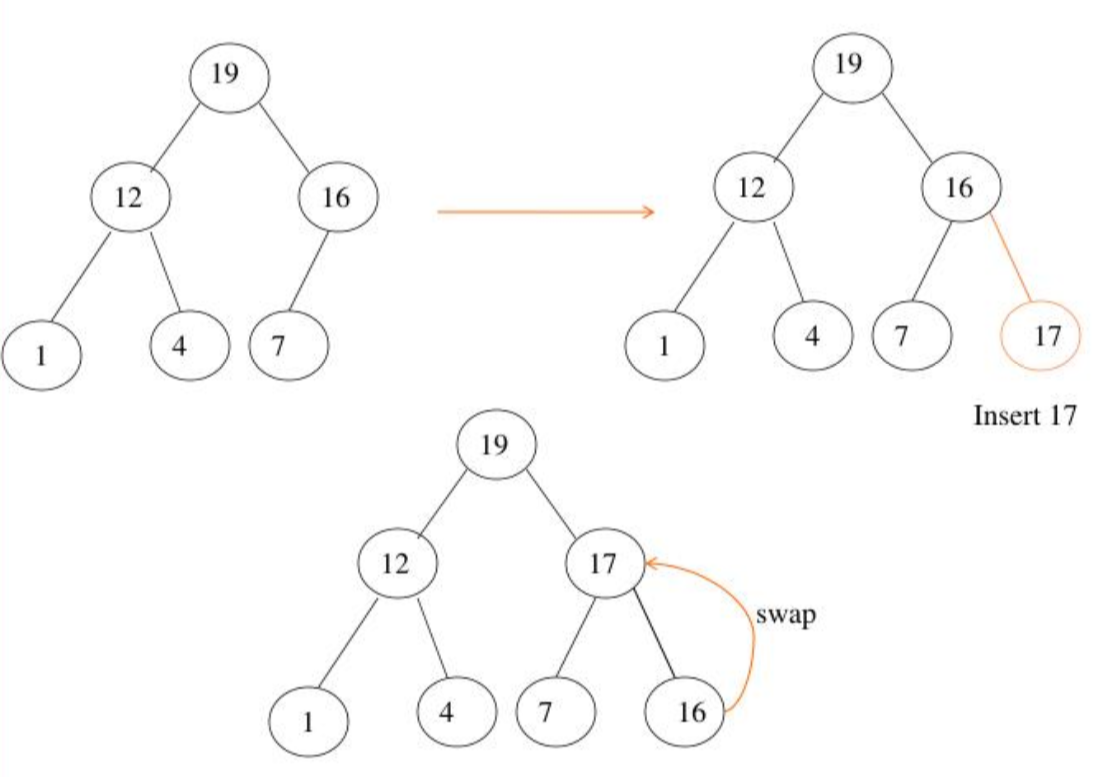
\includegraphics[width=0.5\textwidth]{figs/insert_example.png}};
	\pause
	\node at (3,-2) [color=blue]{$O(\lg{n})$};
	\end{tikzpicture}

	\begin{itemize}
		\item \textbf{\color{blue}Step-1}: \red{Add} the new element to the \teal{end} of the heap
		\item \textbf{\color{blue}Step-2}: \red{Compare} the new element to its \teal{parent}, if it is greater than its parent, \red{swap} the two elements
		\item \textbf{\color{blue}Step-3}: \red{Repeat} step-2 until the new element is smaller than its parent or it is the root.
	\end{itemize}
\end{center}
\end{frame}

\subsection{Inserting an element}
\begin{frame}
\frametitle{Build heap with insertion?}
\begin{center}
	\begin{itemize}
		\item Insert $A[1,..,n]$ to a heap  one by one.
		\item Complexity?
	\end{itemize}
\end{center}
\end{frame}

\subsection{Deleting an element}
\begin{frame}
\frametitle{Deleting an element from a Heap}
Assume that we try to delete a node $i$
\begin{center}
	\pause
	\begin{itemize}
		\item \textbf{\color{blue}Step-1}: \red{Copy} the value of the \teal{last} node  to node $i$ 
		\item \textbf{\color{blue}Step-2}: \red{Remove} the last node
		\item \textbf{\color{blue}Step-3}: \red{Call} \textproc{Max-Heapify} on node $i$
	\end{itemize}

	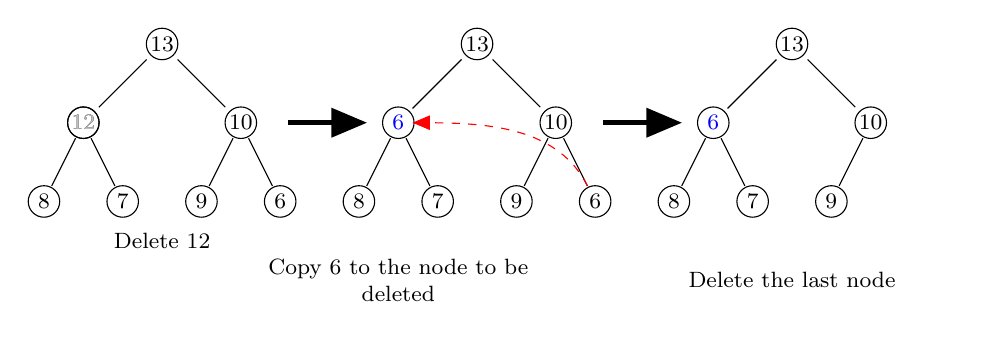
\begin{tikzpicture}
	%init
	\footnotesize{
		\draw (0,0) circle  (0.2) node(n1){13};
		\draw (-1,-1) circle  (0.2) node(n2){12};
		\draw (1,-1) circle  (0.2) node(n3){10};
		\draw (-1.5,-2) circle  (0.2) node(n4){8};
		\draw (-0.5,-2) circle  (0.2) node(n5){7};
		\draw (0.5,-2) circle  (0.2) node(n6){9};
		\draw (1.5,-2) circle  (0.2) node(n7){6};
		\draw (n1)--(n2);
		\draw (n1)--(n3);
		\draw (n2)--(n4);
		\draw (n2)--(n5);
		\draw (n3)--(n6);
		\draw (n3)--(n7);
		\pause
		\node at (0,-2.5){Delete 12};		
		\draw (-1,-1) circle  (0.2) node[color=lightgray]{12};
	}

	\pause
		\draw [->,>=triangle 45, line width=2pt](1.6,-1)--+(1,0);
	\footnotesize{
		\draw [xshift=4cm] (0,0) circle  (0.2) node(n1){13};
		\draw [xshift=4cm] (-1,-1) circle  (0.2) node(n2)[color=blue]{6};
		\draw [xshift=4cm] (1,-1) circle  (0.2) node(n3){10};
		\draw [xshift=4cm] (-1.5,-2) circle  (0.2) node(n4){8};
		\draw [xshift=4cm] (-0.5,-2) circle  (0.2) node(n5){7};
		\draw [xshift=4cm] (0.5,-2) circle  (0.2) node(n6){9};
		\draw [xshift=4cm] (1.5,-2) circle  (0.2) node(n7){6};
		\draw [xshift=4cm] (n1)--(n2);
		\draw [xshift=4cm] (n1)--(n3);
		\draw [xshift=4cm] (n2)--(n4);
		\draw [xshift=4cm] (n2)--(n5);
		\draw [xshift=4cm] (n3)--(n6);
		\draw [xshift=4cm] (n3)--(n7);
		\draw[xshift=4cm,color=red,dashed,->,>=triangle 45] (n7) .. controls (n3) and (0,-1) .. (n2); 
		\node [xshift=3cm]at (0,-3){\parbox{4cm}{\centering{Copy 6 to the node to be deleted}}};		
	}
	\pause
	\draw [xshift=4cm,->,>=triangle 45, line width=2pt](1.6,-1)--+(1,0);
	\footnotesize{
		\draw [xshift=8cm] (0,0) circle  (0.2) node(n1){13};
		\draw [xshift=8cm] (-1,-1) circle  (0.2) node(n2)[color=blue]{6};
		\draw [xshift=8cm] (1,-1) circle  (0.2) node(n3){10};
		\draw [xshift=8cm] (-1.5,-2) circle  (0.2) node(n4){8};
		\draw [xshift=8cm] (-0.5,-2) circle  (0.2) node(n5){7};
		\draw [xshift=8cm] (0.5,-2) circle  (0.2) node(n6){9};
		\draw [xshift=8cm] (n1)--(n2);
		\draw [xshift=8cm] (n1)--(n3);
		\draw [xshift=8cm] (n2)--(n4);
		\draw [xshift=8cm] (n2)--(n5);
		\draw [xshift=8cm] (n3)--(n6);
		\node [xshift=8cm]at (0,-3){\parbox{4cm}{\centering{Delete the last node}}};	
	}
	\end{tikzpicture}
\end{center}
\end{frame}

\section{Heapsort}
\begin{frame}
\frametitle{Heapsort}
\begin{center}
	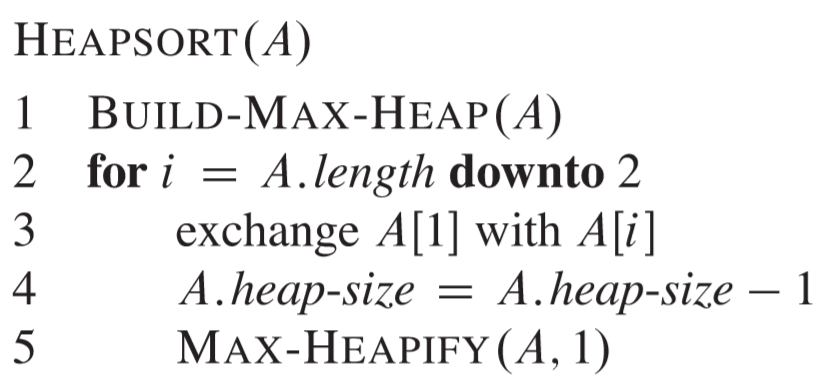
\includegraphics[width=0.5\textwidth]{figs/heapsort_procedure.png}
	
	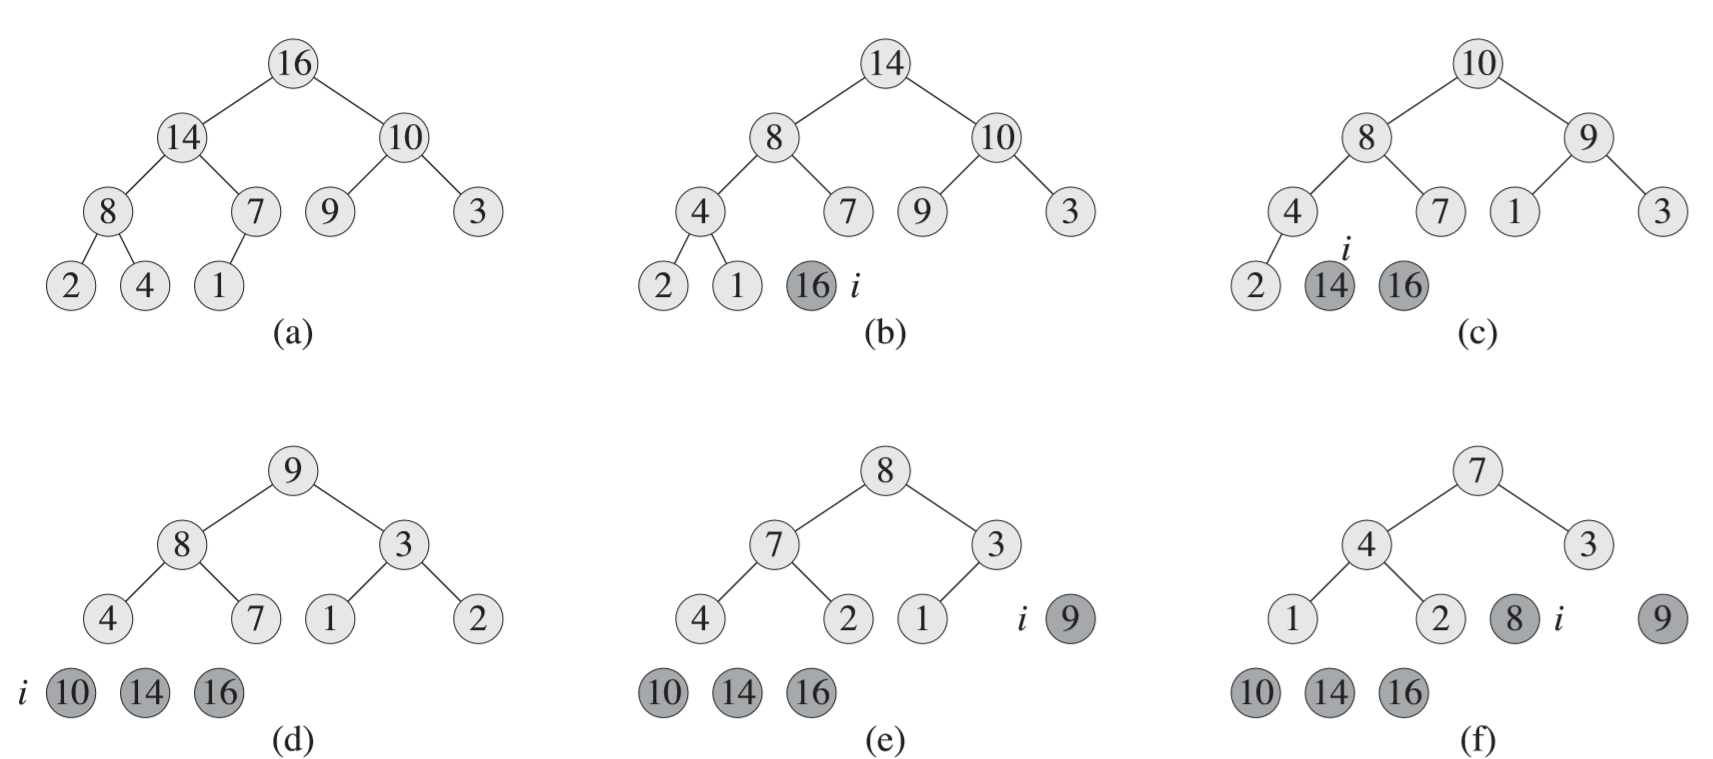
\includegraphics[width=0.9\textwidth]{figs/heapsort_example.png}
\end{center}
\end{frame}
\begin{frame}
\frametitle{Heapsort: Correctness}
\begin{center}
	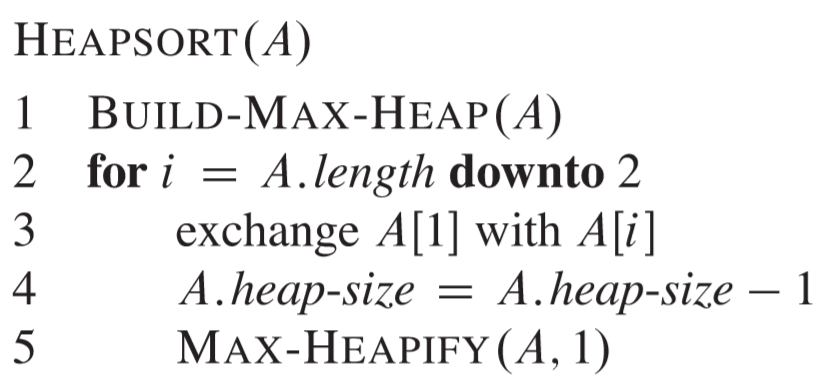
\includegraphics[width=0.5\textwidth]{figs/heapsort_procedure.png}
	
	\question{6}{How to prove the correctness of \textproc{Heapsort}?}
	
	\pause
	\begin{block}{Loop Invariant (\teal{Exercise 6.4-2})}
		\fbox{\parbox{\textwidth}{At the start of each iteration of the for loop of lines 2-5,
		\begin{itemize}
			\item the subarray \teal{$A[1..i]$} is a max-heap containing the $i$ smallest elements of $A[1..n]$,
			\item the subarray \teal{$A[i+1..n]$} contains the $n-i$ largest elements of $A[1..n]$, \red{sorted}.
		\end{itemize}
				 
		}}
	\end{block}
\end{center}
\end{frame}

\begin{frame}
\frametitle{In-place sorting}
\begin{center}
	\begin{block}{In-place sorting algorithms}
		Algorithms require {\color{blue}$O(1)$} extra space and sorting is said to be
		happened in-place, or for example, within the array itself. 
		\pause
		\begin{itemize}
			\item \textproc{Bubble-sort} {\color{green}\cmark}
			\item \textproc{Insertion-sort} {\color{green}\cmark}
			\item \textproc{Heapsort} {\color{green}\cmark}
			\item \textproc{Mergesort} {\color{green}\cmark}
			\item \textproc{Quicksort}{\color{red}\xmark}
		\end{itemize}
	\end{block}
\end{center}
\end{frame}

\begin{frame}
\frametitle{Review \textproc{Quicksort}}
\begin{center}

	\question{7}{Why is \textproc{Quicksort} more efficient in practice?}
	\pause
	\begin{block}{Based on a \textbf{fix computer model}!}
		\begin{itemize}
			\item \textproc{QuickSort}: $11.667(n+1)\ln{n}-1.74n-18.74$
			\item \textproc{MergeSort}: $12.5n\ln{n}$
			\item \textproc{HeapSort}: $16n\ln{n}+0.01n$
			\item \textproc{InsertionSort}: $2.25n^2+7.75n-3\ln{n}$
		\end{itemize}
	\end{block}
	\begin{tikzpicture}
	\node at(-4,0){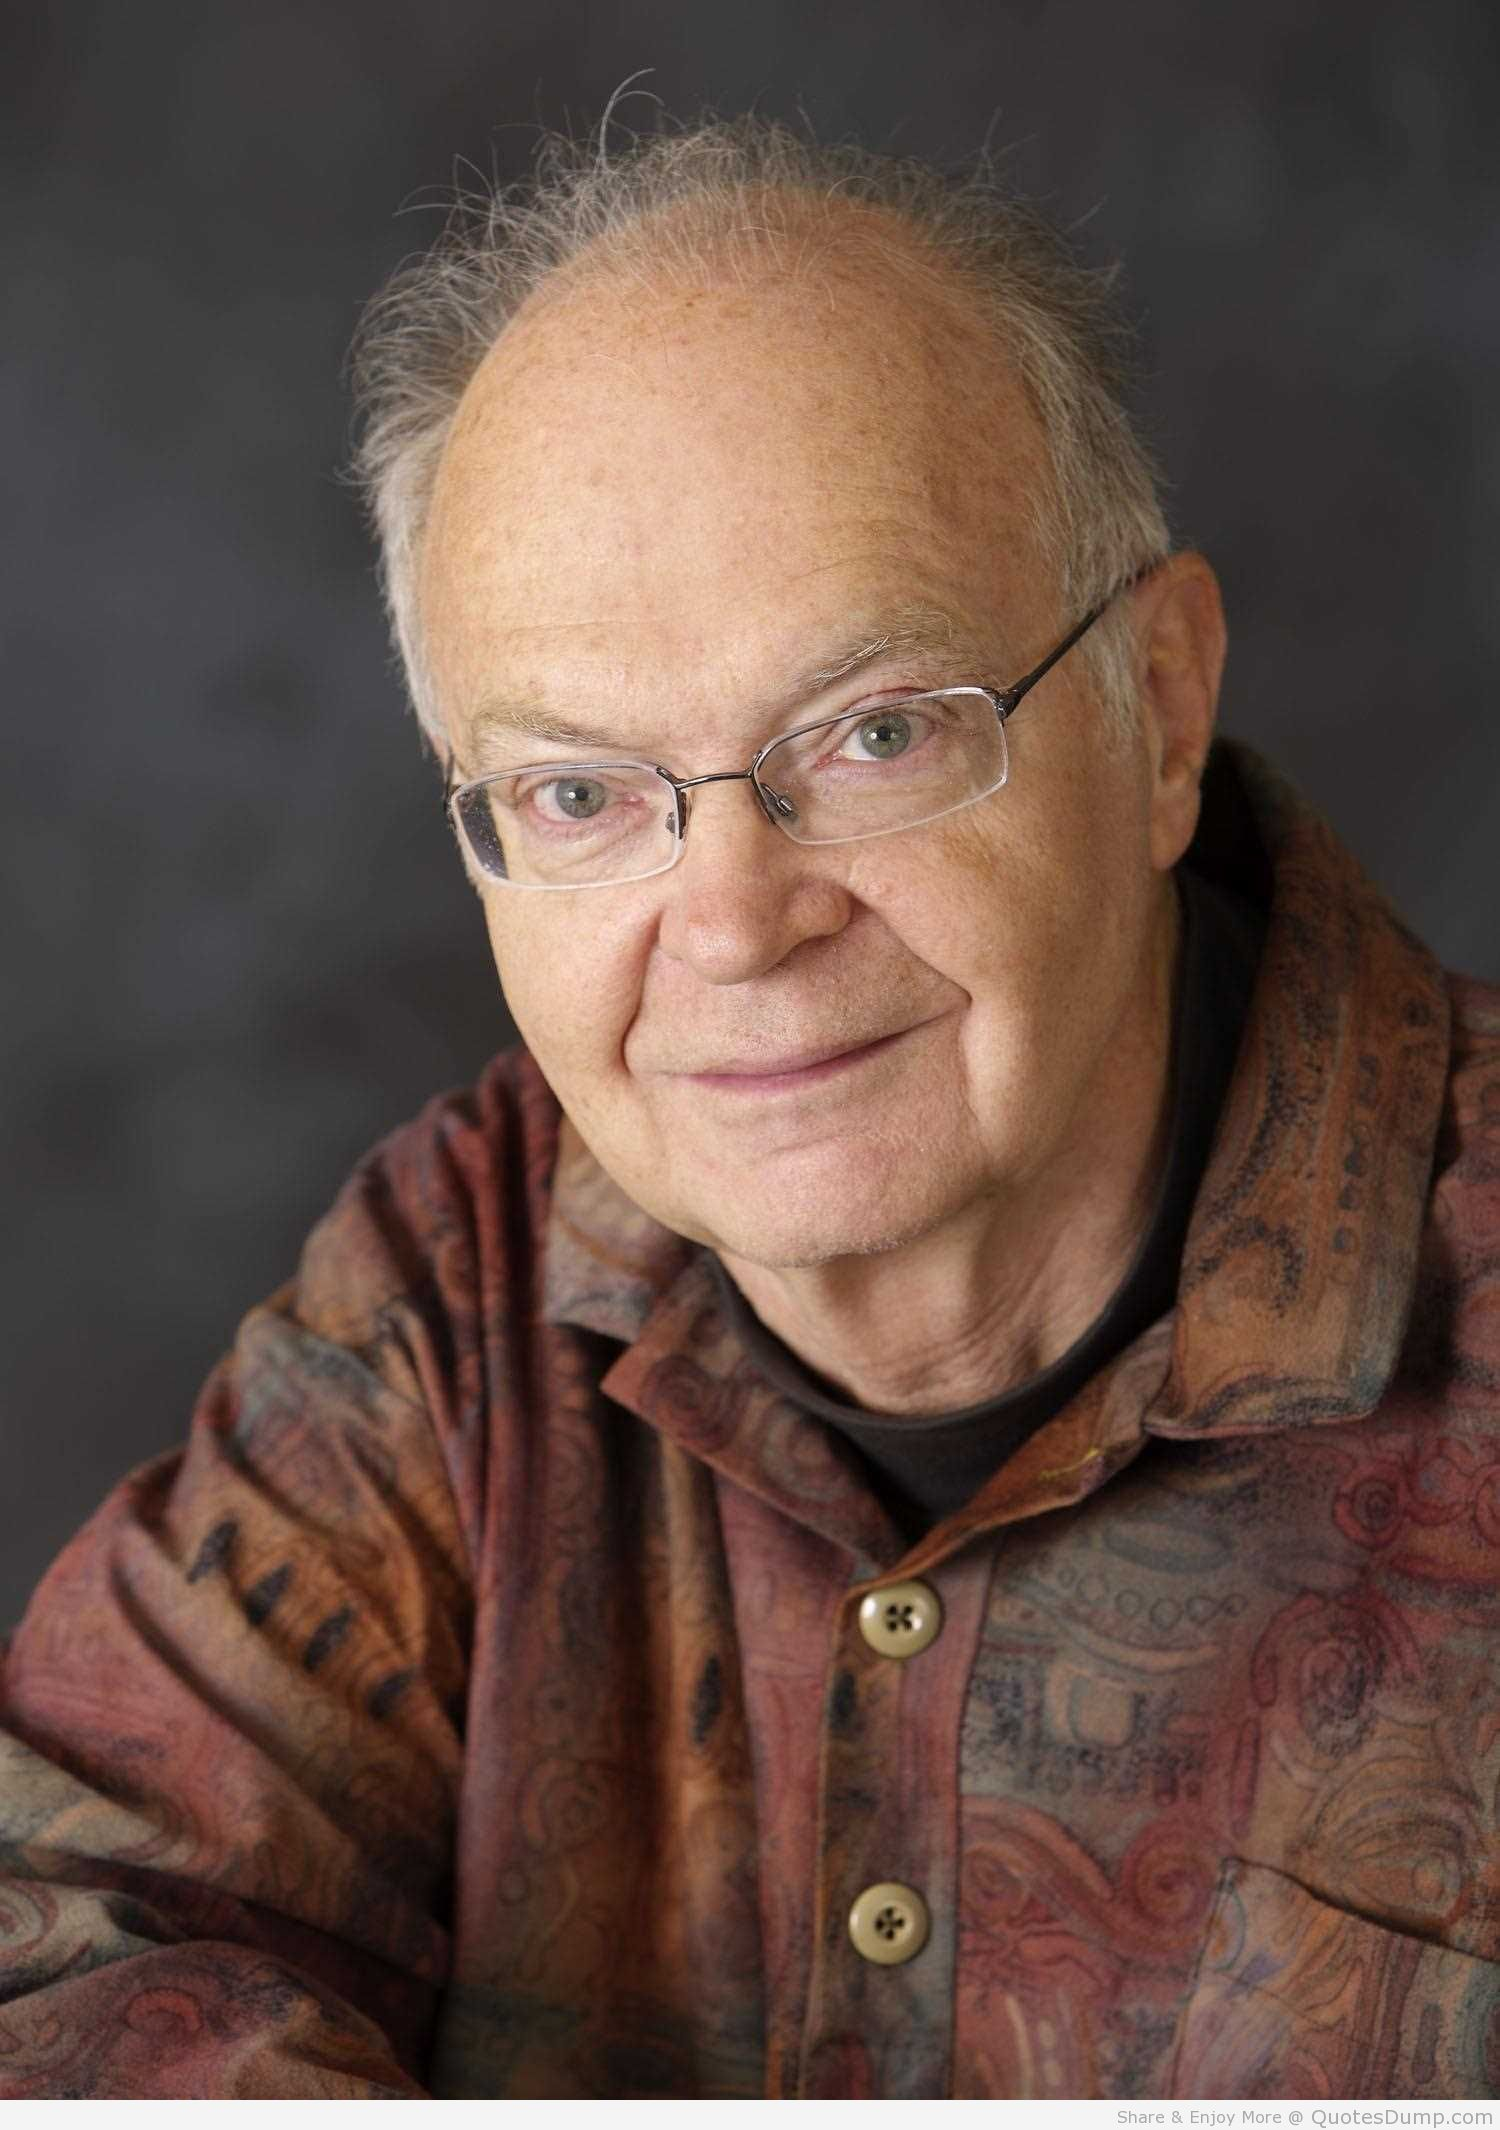
\includegraphics[width=0.15\linewidth]{figs/Donald-Knuth.jpg}};
	\node at(-4,-1.5) {Donald Knuth};
	\node at (0,0) {
\includegraphics[width=0.18\linewidth]{figs/TAOCP_V3.png}};
	\node at (1,-2) {\tiny{\href{https://www-cs-faculty.stanford.edu/\%7Eknuth/taocp.html}{https://www-cs-faculty.stanford.edu/~knuth/taocp.html}}};
	\end{tikzpicture}
\end{center}
\end{frame}

\begin{frame}
\frametitle{Review \textproc{Quicksort}}
\begin{center}
	
	\question{7}{Why is \textproc{Quicksort} more efficient in practice?}
	
	\begin{block}{Analyze \textbf{abstract basic operations}! \teal{\#swap \& \#comparison}}
		
		\begin{itemize}
			\item \textproc{QuickSort}:  $2n\ln{n}$ comparisons and $\frac{1}{3}n\ln{n}$ swaps on average
			\item \textproc{MergeSort}: $1.44n\ln{n}$ comparisons, but up to $8.66nln(n)$ array accesses (mergesort is not swap based, so we cannot count that).
			\item \textproc{InsertionSort}: $\frac{1}{4}n^2$ comparisons and $\frac{1}{4}n^2$ swaps on average.
		\end{itemize}
	\end{block}
	\begin{tikzpicture}
		\node at(-4,0){\includegraphics[width=0.15\linewidth]{../../Homework/2-9-sorting-and-selection/figs/robert-sedgewick}};
		\node at(-4,-1.5) {Robert Sedgewick};
		\node at (0,0) {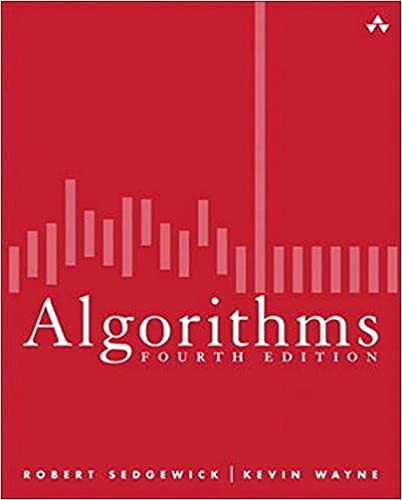
\includegraphics[width=0.2\linewidth]{figs/Book_Algorithms.jpg}};
		\node at (1,-2) {\tiny{\href{https://algs4.cs.princeton.edu/home/}{https://algs4.cs.princeton.edu/home/}}};
	\end{tikzpicture}
	
\end{center}
\end{frame}

\section{Priority Queue}
\begin{frame}[t]
\frametitle{Priority Queue: ADT}
\begin{center}
	\begin{block}{\textbf{Priority queue}}
		A  data structure for maintaining a set $S$ of elements, each with an associated value called a {\color{red}key}.
	\end{block}
	\pause
	\begin{block}{A \textbf{max-priority queue} supports the following operations:}
		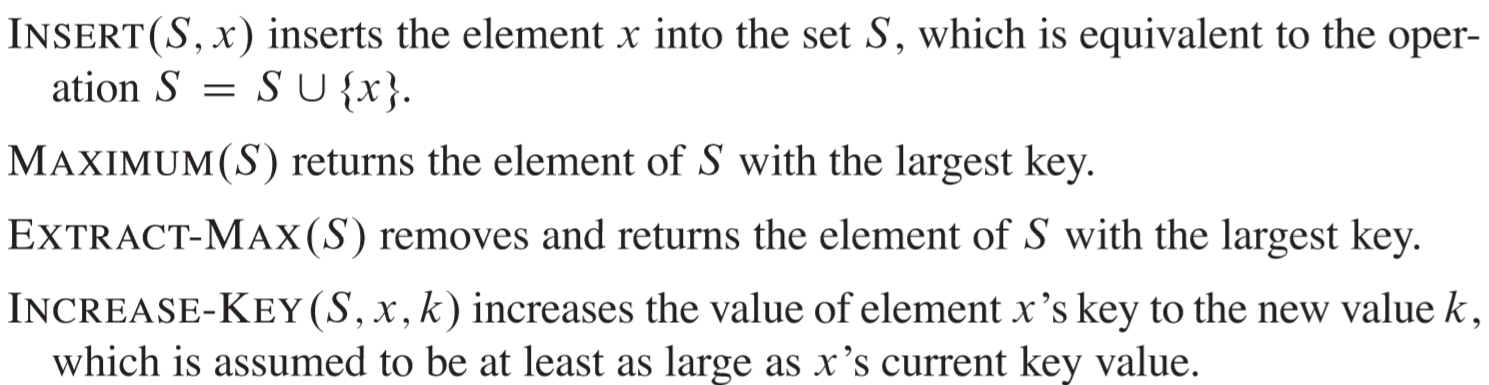
\includegraphics[width=0.9\textwidth]{figs/priority_queue_operations.png}
	\end{block}
\end{center}
\end{frame}

\begin{frame}[t]
\frametitle{Priority Queue: ADT}
\begin{center}
	\question{8}{What is key difference between a Queue and a Priority-queue?}
\end{center}
\begin{columns}
	\begin{column}[T, onlytextwidth]{.45\textwidth}
		\begin{block}{Queue}
			\textbf{\teal{FIFO}}: First-In-First-Out
		\end{block}
		
	\end{column}
	\begin{column}[T, onlytextwidth]{.45\textwidth}
		\begin{block}{Priority Queue}
			\begin{itemize}
				\item \teal{Order} does not matter
				\item \teal{Priority} matters
			\end{itemize}
		\end{block}
	\end{column}
\end{columns}
\end{frame}


\begin{frame}[t]
\frametitle{Priority Queue: Implementation}
\begin{center}
	\begin{block}{ Heap $\rightarrow$ Priority Queue}
	\end{block}
	\begin{tikzpicture}
	\node at(-4,3) {\fbox{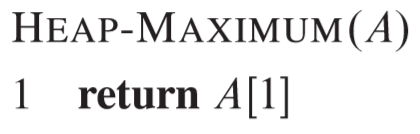
\includegraphics[width=0.25\textwidth]{figs/pq_heap_maximum.png}}};
	\node at(-4,0) {\fbox{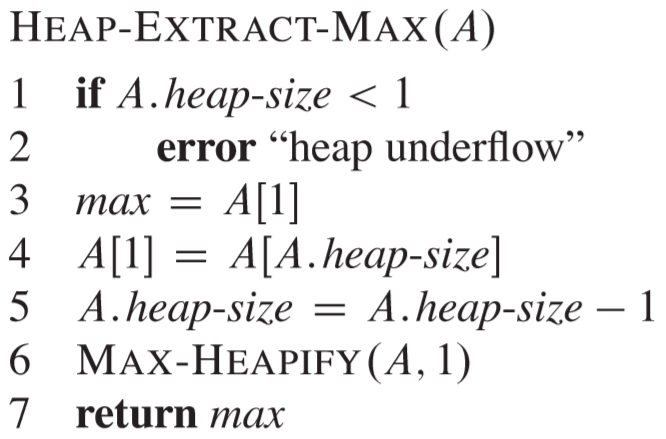
\includegraphics[width=0.4\textwidth]{figs/pq_HEAP-EXTRACT-MAX.png}}};
	\node at(2,2.2) {\fbox{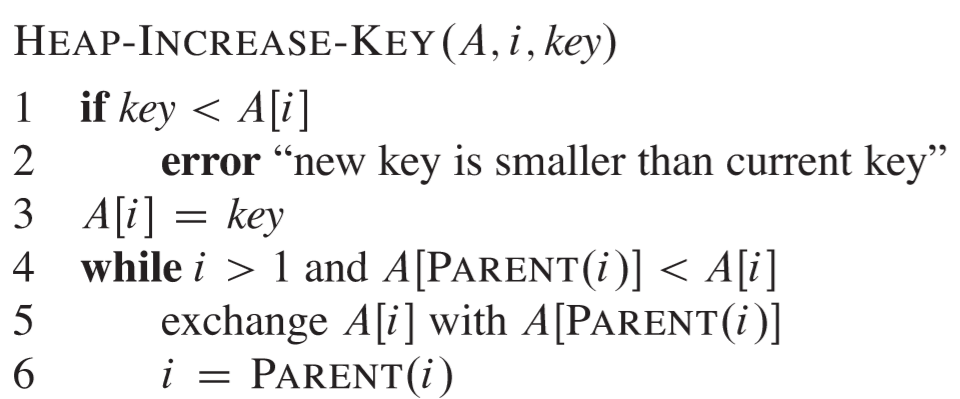
\includegraphics[width=0.5\textwidth]{figs/pq_HEAP-INCREASE-KEY.png}}};
	\node at(2,-0.8) {\fbox{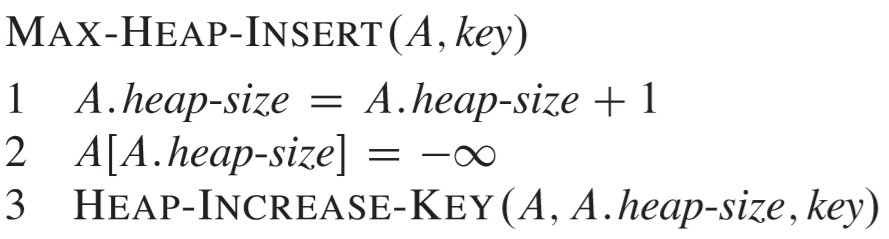
\includegraphics[width=0.5\textwidth]{figs/pq_MAX-HEAP-INSERT.png}}};
	\end{tikzpicture}
\end{center}
\end{frame}

\begin{frame}[t]
\frametitle{Priority Queue: Applications}

\begin{block}{Message Queue}
	In the cloud, a message queue is typically used to delegate tasks to background processing. 
	\begin{center}
		\begin{tikzpicture}
		\node at(0,0){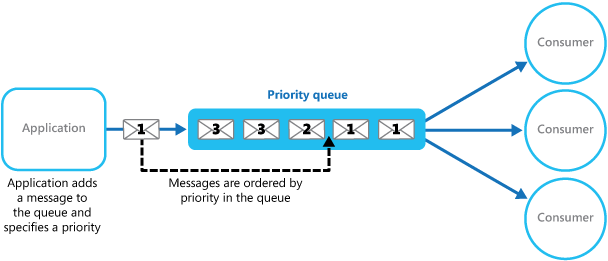
\includegraphics[width=0.9\linewidth]{figs/priority-queue-pattern.png}};
		\node at(0,-3){\tiny{\href{https://docs.microsoft.com/en-us/azure/architecture/patterns/priority-queue}{https://docs.microsoft.com/en-us/azure/architecture/patterns/priority-queue}}};
		\end{tikzpicture}	
	\end{center}
\end{block}
\end{frame}

\begin{frame}[t]
\frametitle{Priority Queue: Applications}
\begin{block}{Message Queue (Without Priority Queue)}
	\begin{center}
		\begin{tikzpicture}
		\node at(0,0){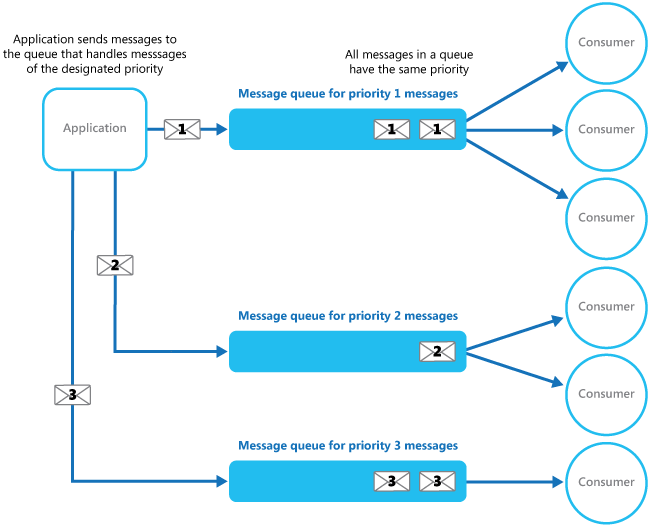
\includegraphics[height=0.7\textheight]{figs/priority-queue-separate.png}};
		\node at(0,-3){\tiny{\href{https://docs.microsoft.com/en-us/azure/architecture/patterns/priority-queue}{https://docs.microsoft.com/en-us/azure/architecture/patterns/priority-queue}}};
		\end{tikzpicture}	
	\end{center}
\end{block}
\end{frame}

\begin{frame}[t]
\frametitle{Priority Queue: Applications}
\begin{block}{Dijkstra's Shortest Path Algorithm}
	\begin{center}
		\begin{tikzpicture}
		\node at(-5,0){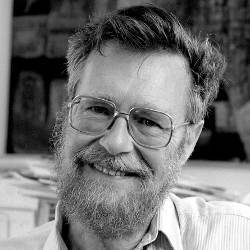
\includegraphics[width=0.2\linewidth]{figs/dijkstra.jpg}};
		\node at(-5,-2){\parbox{3cm}{\scriptsize{ Edsger W. Dijkstra.\\
					1972 ACM A.M. Turing Award winner}}};
		\node at(0,0){	\animategraphics[autoplay,loop,width=0.35\textwidth]{3}{figs/Dijkstra_Animation-}{0}{42}};
		\node at(0,-2.5){\tiny{\href{https://en.wikipedia.org/wiki/Dijkstra\%27s\_algorithm}{https://en.wikipedia.org/wiki/Dijkstra\%27s\_algorithm}}};
		\end{tikzpicture}	
	\end{center}
	\footnotesize{\blue{``I designed in about twenty minutes''}.
		
		In 1956, ``One morning I was shopping in Amsterdam with my young fiancée, and tired, we sat down on the café terrace to drink a cup of coffee and I was just thinking about whether I could do this, and I then designed the algorithm for the shortest path''}
\end{block}
\end{frame}

\begin{frame}[t]
\frametitle{Priority Queue: Applications}
\begin{block}{Prim Algorithm for MST}
	\begin{center}
		\begin{tikzpicture}
		\node at(0,0){	\animategraphics[autoplay,loop,width=0.4\textwidth]{3}{figs/PrimAlgDemo-}{0}{57}};
		\node at(0,-3){\tiny{\href{https://en.wikipedia.org/wiki/Dijkstra\%27s\_algorithm}{https://en.wikipedia.org/wiki/Dijkstra\%27s\_algorithm}}};
		\end{tikzpicture}	
	\end{center}
\end{block}
\end{frame}


\begin{frame}
	\begin{block}{
		\begin{center}
		{\huge
			Thank You!
			
			\textcolor[rgb]{1,0,0}	{Questions?}
		}
		\end{center}
	}
	\end{block}
	\begin{block}{}
		\begin{center}
		
			Office 819
			
			majun@nju.edu.cn
		\end{center}
	\end{block}
	\end{frame}
\end{document}